\documentclass[11pt,a4]{article}
\usepackage[cm]{fullpage}
\usepackage{graphicx}
\usepackage{subfigure}
\usepackage{epsfig}
\usepackage{epstopdf}
\begin{document}

\begin{figure}[h]
\centering
    \includegraphics[width=0.49\textwidth]{FOS}
    \includegraphics[width=0.49\textwidth]{GATA2}
    \includegraphics[width=0.49\textwidth]{MYC}
    \includegraphics[width=0.49\textwidth]{JUN}
\caption{ROC curve created when applying the methods to data from the cell line Huvec. All HMM Models were trained with data from H1-hESC and K562 cell lines.}
\label{fig:roc.Huvec.1}
\end{figure}

\begin{figure}[h]
\centering
    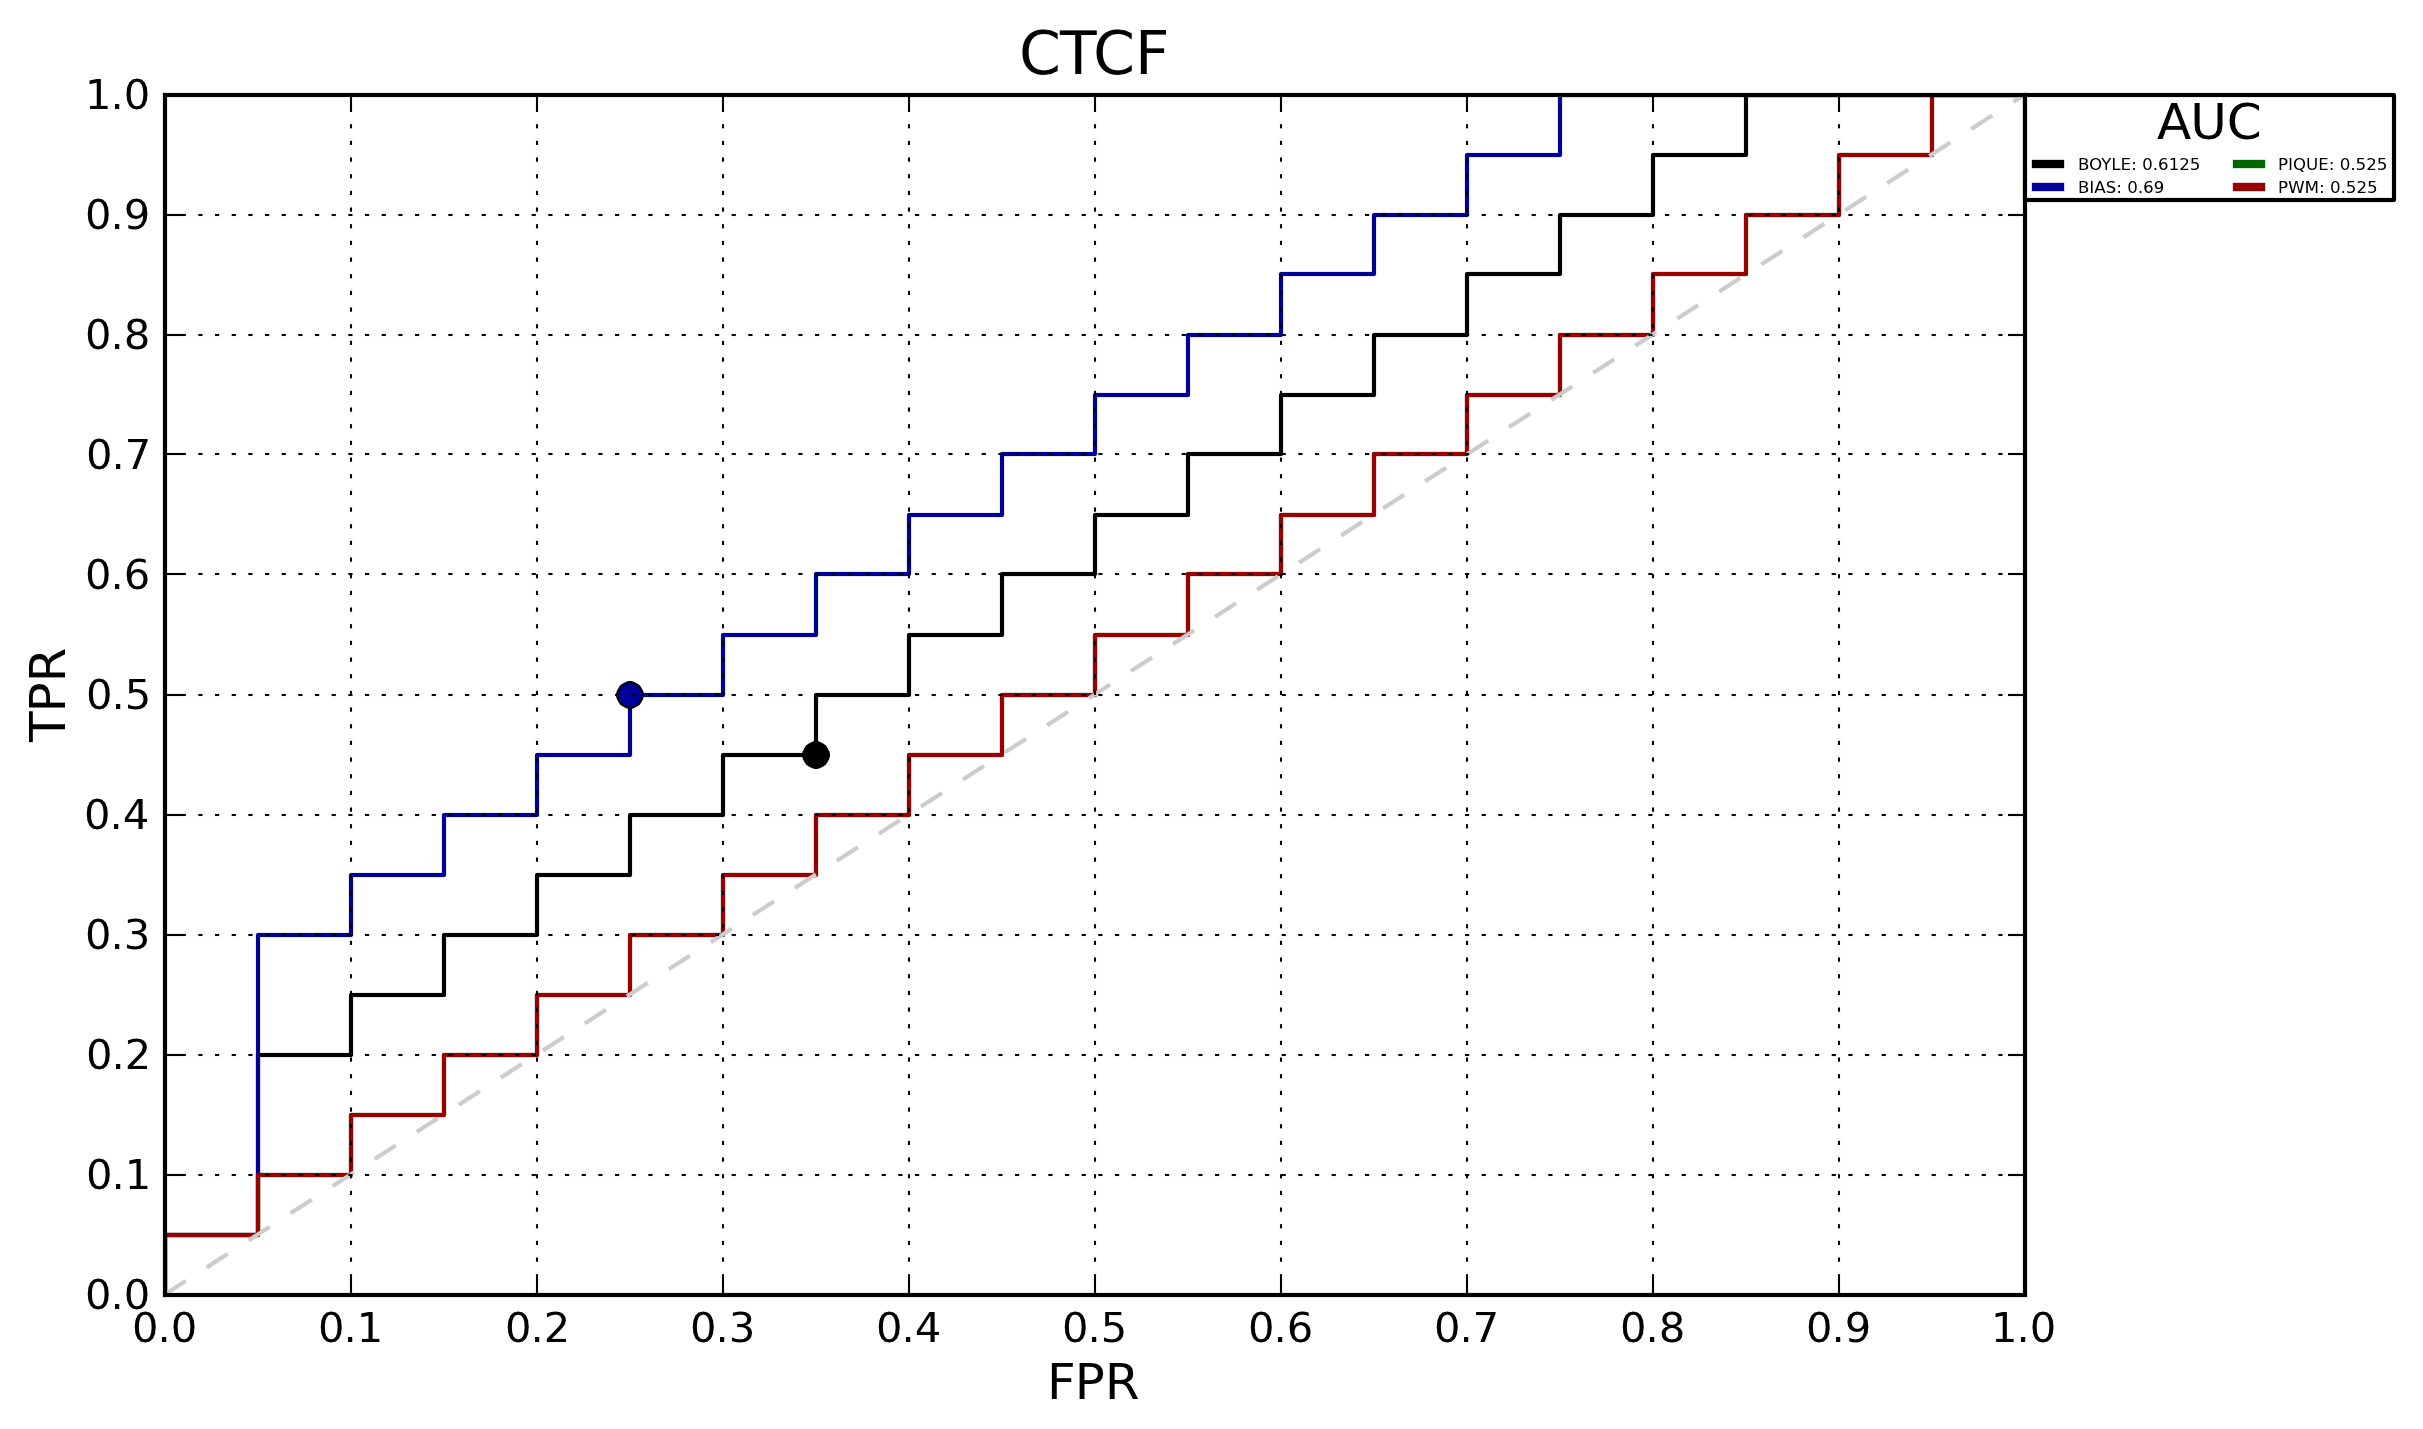
\includegraphics[width=0.49\textwidth]{CTCF}
    \includegraphics[width=0.49\textwidth]{MAX}
\caption{ROC curve created when applying the methods to data from the cell line Huvec. All HMM Models were trained with data from H1-hESC and K562 cell lines.}
\label{fig:roc.Huvec.2}
\end{figure}

\end{document}